
\documentclass[aps,twocolumn,pre,nofootinbib,10pt]{revtex4-1}

%\usepackage{auto-pst-pdf}
\usepackage{algcompatible}
\usepackage[noend]{algpseudocode}
\usepackage{graphicx}
\graphicspath{{../plots/}}
\usepackage{amsmath,amssymb,amsfonts,amsthm}
\usepackage{bbm}
\usepackage{newfloat}
\usepackage{times}
\usepackage{float}
\usepackage{array}
\usepackage{esint}

\renewcommand{\thefigure}{\arabic{section}.\arabic{figure}}

\DeclareFloatingEnvironment[
    fileext=loa,
    listname=List of Algorithms,
    name=ALGORITHM,
    placement=tbhp,
]{algorithm}


\begin{document}


%%%%%%%%%%%%%%%%%%%%%%%%%%%%%%%%%%%%%%%%%%%%%%%%%%%%
% Useful symbols and definitions that may save time
%%%%%%%%%%%%%%%%%%%%%%%%%%%%%%%%%%%%%%%%%%%%%%%%%%%%

\newcommand{\breite}{1.0} %  for twocolumn


\newtheorem{prop}{Proposition}
\newtheorem{cor}{Corollary}

\newcommand{\be}{\begin{equation}}
\newcommand{\ee}{\end{equation}}

\newcommand{\bea}{\begin{eqnarray}}
\newcommand{\eea}{\end{eqnarray}}

\newcommand{\Reals}{\mathbb{R}}     % Real
\newcommand{\Int}{\mathbb{Z}}       % Integer
\newcommand{\Com}{\mathbb{C}}       % Complex 
\newcommand{\Nat}{\mathbb{N}}       % Natural 


\newcommand{\id}{\mathbbm{1}}    

\newcommand{\Real}{\mathop{\mathrm{Re}}}
\newcommand{\Imag}{\mathop{\mathrm{Im}}}

\def\O{\mbox{$\mathcal{O}$}}    
\def\F{\mathcal{F}}			
\def\sgn{\text{sgn}}

\newcommand{\dw}{\ensuremath{\Delta}} %I think I have most we need but will add any if needed.
\newcommand{\wbp}{\ensuremath{\omega_0}}
\newcommand{\dv}{\ensuremath{\delta}}
\newcommand{\vbp}{\ensuremath{\nu_0}}
\newcommand{\vplus}{\ensuremath{\nu_{+}}}
\newcommand{\vminus}{\ensuremath{\nu_{-}}}
\newcommand{\wplus}{\ensuremath{\omega_{+}}}
\newcommand{\wminus}{\ensuremath{\omega_{-}}}
\newcommand{\den}{\ensuremath{\rho}}
\newcommand{\del}{\ensuremath{\nabla}}
\newcommand{\per}{\ensuremath{\epsilon_0}}
\newcommand{\pot}{\ensuremath{\phi}}
\newcommand*\Let[2]{\State #1 $\gets$ #2}
%%%%%%%%%%%%%%%%%%%%%%%%%%%%%%%%%%%%%%%%%%%%%



%Title of paper (I know it isn't very creative but it isn't supposed to be. We can definitely discuss this! 
\title{Numerical solutions to the Laplace Equation applied to electrostatic fields}


%Us
\author{Karl Nordstorm}

\author{David Muir}

\author{Julia Kettle}

\author{John Maccorquodale}

\author{Jevgeny Klochan}

\author{Stephen Shepstone}


\affiliation{University Of Glasgow}

\date{\today}
%%%%%%%%%%%%%%%%%%%%%%%%%%%%%%%%%%%%%%%%%%%%%%%%%%%%

%ABSTRACT
\begin{abstract}

Abstract... 
  
\end{abstract}


%FINISH TITLE
\maketitle


%INTRODUCTION

\section{Introduction \label{sec:int}}

Computational Physics is an important part of modern physics. It has uses in a wide range of fields such as astrophysics, particle physics, lattice QCD, and is generally used across all of theoretical physics. Applications include quantum mechanical calculations involving atomic, molecular and condensation physics, modelling in medical physics and industry, and calculations involving fields in hydrodynamics, thermal physics, astrophysics, meteorology, lattice QCD, and geophysics. 
Specifically computational physics can be applied to differential equations, with many applications in fields mentioned above, as well as in classical electromagnetism.
Consider a stationary zero net-charge conducting cylinder in a uniform electrostatic field as shown in figure (\ref{fig:fig1}). The divergence of the electric field would be:

\begin{gather}
  \vec{\del}.\vec{E}= \frac{\den}{\per} 
\label{fig:eqn1}
\end{gather}

by Gauss' law where $\del$ is the differential operator, $\vec{E}$ is the electric field, $\den$  is the charge density and $\per$ is the permittivity of free space.

As charge is redistributed to either side of the conductor, the electric fields close to the conductor are warped: negative side will become a sink, whereas the positive side will become a source since $\den$ will be negative and positive, respectively around these areas. For points outside the space filled by the conductor, there will be a zero charge density. This implies that the solution for figure (\ref{fig:fig1}) is reduced to:

\begin{gather}
\vec{\del}.\vec{E}= 0 
\label{fig:eqn2}
\end{gather}

for all points outside the conductor. It is also the case that the field will be conservative and can therefore be written as a scalar potential with:

\begin{gather}
\vec{E}= -\del\Phi.
\label{fig:eqn3}
\end{gather}

Combining (\ref{fig:eqn2}) and (\ref{fig:eqn3}) gives:

\begin{gather}
\del^2\Phi=0
\label{fig:eqn4}
\end{gather}

Hence, the solution to the problem is given by the Laplace Equation.

\begin{figure}[h]
\includegraphics*[height=\breite \columnwidth,angle=270]{first_plot.ps} 
\caption{Cross section of zero net charge circular conductor in uniform electrostatic field. The colours are used to show the potential at each point, and the lines show points of equipotential.}
\label{fig:fig1}
\end{figure}

 

%THEORY AND ALGORITHMS
\section{Theory \label{sec:the}}

\subsection{Solving the Laplace Equation in two dimensions}
We'll solve Laplace's Equation in polar coordinates for the scalar field $\Phi(r, \theta)$:
\[ \left( r \Phi_r \right)_r + \frac{1}{r} \left(\Phi_\theta \right)_\theta = 0 \]
Assuming we can separate variables such that $\Phi(r, \theta) = R(r)\Theta(\theta)$:
\begin{gather*}
 \Phi_r = R'\Theta, \Phi_\theta = R\Theta' \Rightarrow \\
 (rR'\Theta)_r + \frac{1}{r}(R\Theta')_\theta = 0 \Leftrightarrow \\
 R'\Theta + rR''\Theta + \frac{1}{r}R\Theta'' = 0 \Leftrightarrow \\
 \frac{rR' + r^2 R''}{R} = \frac{- \Theta''}{\Theta} \Leftrightarrow \\
 \frac{r(rR')'}{R} = \frac{- \Theta''}{\Theta}
\end{gather*}

Set both sides equal to $\lambda^2$:
\[ (A) \hspace{0.5cm} \frac{r(rR')'}{R} = \lambda^2, \hspace{1cm} (B) \hspace{0.5cm} \frac{- \Theta''}{\Theta} = \lambda^2 \]
Solve the two differential equations separately, assuming at first that $\lambda \neq 0$. For (A), we can guess that the solution takes a familiar form $R(r) = \gamma r^\alpha$:
\begin{gather*}
 R' = \gamma \alpha r^{\alpha - 1} \Rightarrow \\
 \frac{r(r\gamma \alpha r^{\alpha - 1})'}{\gamma r^\alpha} = \lambda^2 \Leftrightarrow \\
 \alpha^2 \frac{\gamma r r^{\alpha - 1}}{\gamma r^\alpha} = \lambda^2 \Leftrightarrow \\
 \alpha^2 = \lambda^2 \Rightarrow \alpha = \pm \lambda 
\end{gather*}
For (B), we have $\Theta'' + \lambda^2 \Theta = 0$, so the general form of the solution is:
\[ \Theta(\theta) = A \cos(\lambda \theta) + B \sin(\lambda \theta) \]
Since $\Theta(0) = \Theta(2\pi)$ we know that $\lambda \in \mathbb{N}$ (or, more generally,
that $\lambda \in \mathbb{Z}$ but due to the symmetry in $\cos$ and $\sin$ that information can be encoded into $A$ and $B$).
When $\lambda = 0$ we can in both cases integrate to find the solutions:
\[ (A) \hspace{0.5cm} R(r) = c_1 \ln r + c_2,\hspace{1cm} (B)\hspace{0.5cm} \Theta(\theta) = c_3 \theta + c_4 \]
Since the Laplace Equation is linear, we can add the solutions together to get the general solution set, using the assumption that they are separable:
\begin{gather}
 \Phi(r, \theta) = R(r)\Theta(\theta)_{\lambda = 0} + R(r)\Theta(\theta)_{\lambda \in \mathbb{N}} = \nonumber \\
 (c_1 \ln r + c_2)(c_3 \theta + c_4) + \nonumber \\ 
\sum_{n \in \mathbb{N}} (\gamma_{1n} r^n + \gamma_{2n} r^{-n})
\big[A \cos(n \theta) + B \sin(n \theta) \big] \label{generalsol}
\end{gather}

\subsection{Particular solution for infinite cylinder in $\vec{E}$ field}
We will add two different solutions together to find the total potential. Let the $\vec{E}$ field be uniform in the x direction
such that $\vec{E} = E_0 \hat{x}$. Since $\vec{E} = - \nabla \Phi$, $\Phi = -E_0 x = -E_0 r \cos\theta$, which is
in the general solution set (\ref{generalsol}) we derived above.
Our first
boundary condition is then:
\[ \lim_{r \rightarrow \infty} \Phi(r,\theta)_{total} = -E_0 r \cos\theta \]
Next we want to find the field from the cylinder. Let the radius of the cylinder be $R$.
The second boundary condition is that the potential on the surface of the cylinder must be constant,
say $V_0$, so:
\[ (C) \hspace{0.5cm} \Phi(R,\theta)_{total} = -E_0 R \cos\theta + \Phi(R,\theta)_{cylinder} = V_0 \]
$\Phi(r,\theta)_{cylinder}$ must also be in the general solution set defined above. We need a constant so take $c_2 c_4$ from the first
part of the general solution, but discard the
$\ln r$ and $\theta$ terms to keep within the first boundary condition.
From the second part we need to get an expression which lets us fulfill (C), so it is logical to take the $n = 1$ term which has $\cos\theta$:

\begin{gather*}
 \Phi(R,\theta)_{total} = -E_0 R \cos\theta +  c_2 c_4 + \\
(\gamma_{11} R + \gamma_{21} R^{-1}) (A\cos\theta + B \sin\theta) = V_0 
\end{gather*}

Now $B$ must be zero since the sin term would violate the symmetry we require about the x axis, and all that is left is to solve the following equation:

\begin{gather*}
 \Phi(R,\theta)_{total} = -E_0 R \cos\theta + c_2 c_4 + \\
(\gamma_{11} R + \gamma_{21} R^{-1}) A\cos\theta = V_0 \Leftrightarrow \\
 c_2 c_4 - V_0 + R \cos\theta \left( A\gamma_{11} - E_0 + \frac{A\gamma_{21}}{R^2} \right) = 0 
\end{gather*}

Hence set $c_2 c_4 = V_0$, $\gamma_{11} = 0$, and $A\gamma_{21} = E_0 R^2$ to fulfill (C) and get the final solution:
\begin{gather}
 \Phi(r,\theta)_{total} = V_0 + E_0 cos\theta \left( \frac{R^2}{r} - r \right)
 \label{analyticsol}
\end{gather}

\subsection{Conservation of charge}

A powerful tool for investigating the validity of our numerical solutions is conservation of charge. Since we are adding neutral conductors to the field, the total integrated field should not change as a result. To understand how it is possible for some numerical solutions to break this fundamental rule we will first consider the electric potential created by a conductor in the field, and then use the power of gauge theory and Noether's Theorem to qualitatively explain the effect.

As the redistribution of charges in the conductor cancels out the electric field inside it, and it has a total charge of 0, we can approximate the charge distribution in the stable state to be similar to an electric dipole where the charges are separated by the length of the conductor in the direction of the field, $l$. This allows us to derive a mathematical expression for the electric potential caused by it:

Consider two charges, $q_+$ and $q_-$, separated by $l$. The total potential at a point $\vec{r}$, at an angle $\theta$ from the normal to $l$, separated from the charges by $r_+$ and $r_-$ can then be written by:

\begin{gather*}
V(\vec{r}) = V(r_+) + V(r_-) \\
 = \frac{q_+}{4 \pi \epsilon_0 r_+} + \frac{q_-}{4 \pi \epsilon_0 r_-} \\
 = \frac{q}{4 \pi \epsilon_0}\left( \frac{r_- - r_+}{r_+ r_-} \right) \\
\end{gather*}
\begin{gather}
 \approx \frac{q}{4 \pi \epsilon_0} \left( \frac{l \sin\theta}{r^2} \right) 
 \label{dipole}
\end{gather}

Here $r$ is the distance from the midpoint between the two charges to $\vec{r}$. Note that this potential is proportional to $1/r^2$ unlike the electric potential from a point charge, which limits its effective range considerably.

Gauge theory is a powerful tool for analysing fields where the observable quantities are invariant under certain transformations of the field itself \cite{gaugetheory1}. By Noether's two theorems, these symmetries all have corresponding conservation laws: the conserved Noether currents.\footnote{Note that there are two Noether theorems to deal with global and local symmetries separately. Global symmetries always lead to conserved currents, while local symmetries do so under certain conditions. See for example \cite{gaugetheory2}.} The symmetry group of electromagnetism is $U(1)$, and for local gauge invariance requires that its gauge boson is massless and hence gives the force infinite range. Local gauge invariance is here the symmetry that results in conservation of charge. The same symmetry is of course required for the weak force as well, which is why the Higgs mechanism was invented to introduce a way to consistently give mass to the 
$Z$ and $W^{\pm}$ bosons and hence limit the range of the weak force according to experimental observations without breaking gauge invariance \cite{gaugetheory3}. In our case we are interested in gauge theory because it allows us to predict that meaningfully limiting the range of the electromagnetic force by using a finite grid size with the assumption that the conductor won't change the field at the 
boundaries will break conservation of charge. 'Meaningfully' here refers to the fact that the potential from the conductor will tend to 0 quickly as we move further away from it due to the inverse square law, so we can estimate the field to be effectively zero at some finite distance away. This allows us to justify the use of the finite grid sizes we require to make sensible numerical simulations, and gives us a good variable to use for determining how small we can make the grid in comparison to the conductor without creating unphysical solutions: conservation of charge.\footnote{Of course many problems with enough symmetry will obey conservation of charge even though the range is effectively limited. This has to be taken into consideration when using charge conservation to measure the required size of the grid.} The dipole potential calculation (\ref{dipole}) also tells us that the required size of the grid varies roughly linearly with the length $l$ of the conductor in the direction of the field, whereas the size in the 
orthogonal direction to the field is less important.

\subsection{Multiple conductors}
The problem of adding multiple conductors to the same field is that in order to obey charge conservation, they must all take the fields generated by the others into account when deciding their equilibrium potential. Since we haven't implemented a path integral along the surface of the conductor to allow for time-like evolution of the potential of the conductors themselves using Stokes' theorem, we are 'stuck' with the field as the conductor sees it when it is first entered for deciding its potential. In other words, adding one and solving before adding a new one and keeping the old one constant will give an unphysical result, as the first one will affect the second one but we don't have a mechanism for allowing the second one to affect the first one. Figure \ref{fig:difference} shows the difference between a physically correct solution and a solution obtained by the adding the conductors one at a time. The simplest correct way of dealing with this problem is to find solutions for each individual conductor first, averaging them all, and then adding all the conductors into the averaged field at once before solving a last time. This ensures that charge conservation is obeyed and gives the correct physical solution. An alternative solution would be to implement a Stokes integration along the surface of the conductor as outlined above.

\begin{figure}
\includegraphics*[height=\breite \columnwidth,angle=270]{difference.ps} 
\caption{Difference between solutions when two circular conductors are added one at a time and solved simultaneously. A negative value means the solution where conductors are added one at a time is lower than the simultaneous solution. The original uniform field runs from 50 on the left to -50 on the right. An integration over the fields gives a mean charge of about -0.16 in the one at a time solution and effectively 0 in the simultaneous one: a clear indication that charge conservation is violated when adding conductors one at at time.}
\label{fig:difference}
\end{figure}
 

%METHODS- I think algorithms should go here rather than code. Any chunks of code that are necessary for the 
%report should go into the appendix
\section{Numerical Methods \label{sec:met}}

 
\subsection{Finite Difference Method}

\subsubsection{Background Information}

\par\hspace{4mm} In mathematics, there are a number numerical procedures for estimating the solutions to differential equations using finite difference equations to approximate derivatives. These are knowns as finite difference methods. A finite difference is a mathematical expression of the form \(f(x + b) - f(x + a)\). If a finite difference is divided by \((b - a)\), one gets a difference quotient. The estimation of derivatives by finite differences plays a central role in finite difference methods for the numerical solution of differential equations, especially boundary value problems.
\vspace{5mm} \par \indent An essential application of finite differences is in numerical analysis, especially in numerical differential equations, which aim at the numerical solution of ordinary and partial differential equations. The idea is to replace the derivatives appearing in the differential equation by finite differences that approximate them. The resulting methods are called finite difference methods. Other common applications of the finite difference method are in computational science and engineering disciplines, such as thermal engineering and fluid mechanics. Also interestingly recurrence relations can be written as difference equations by replacing iteration notation with finite differences.\footnote{This is perhaps not surprising, as recurrence relations have strong similarities to differential equations. For a formalised approach to this area, see time-scale calculus, which unifies finite difference calculus and differential calculus to form a theory that can deal with systems with both 
continuous and discrete variables.}

\subsubsection{Accuracy of the method}

\par\hspace{4mm} In this paper we define the error as the difference between the approximation and the exact analytical solution, hence we will use simple problems with a lot of symmetry to check the accuracy of our methods. To approximate the solution to a problem when using the finite difference method the domain we want to solve over must first be discretised.\footnote{In short we want to deal with small individual elements rather than a continuous space.} Dividing the domain into a uniform grid is the usual manner of doing this. From this the finite difference method will present various discrete numerical estimations to the derivative. We will only be working with first order approximations, so from this point on we will refer to the first order approximation whenever we talk about the finite difference method.

\subsubsection{Approximation of second order derivative}
Consider the arbitrary function \(f(x)\). The Taylor series of this function centered at the value \(x=a\) is:

\begin{gather*}
f(x) = f(a) +(x-a)f^{(1)}(x)+\frac{(x-a)^{2}f^{(2)}(x)}{2!}+ \\
\frac{(x-a)^{3}f^{(3)}(x)}{3!}+...
\end{gather*}

Center around $x_i$ and let \(x=x_i + h\) then:

\begin{gather*}
f(x_i\pm h)=f(x_i) \pm hf^{(1)}(x_i)+\frac{h^2f^{(2)}(x_i)}{2!} \pm \frac{h^3f^{(3)}(x_i)}{3!}+...
\end{gather*}

Therefore:

\begin{gather*}
f(x_i+h)+f(x_i-h) = 2f(x_i) + h^2f^{(2)}(x_i) +\frac{h^4}{12}f^{(4)}(x_i)+...
\end{gather*}

If h is very small then only the first two terms are significant and the later terms can be ignored to yield a good approximation:

\begin{gather*}
f(x_i+h)+f(x_i-h) \approx 2f(x_i) + h^2f^{(2)}(x_i)
\end{gather*}

So, by rearranging, the second order derivative of a function at \(x_i\) can be approximated by:

\begin{gather*}
\frac{d^2f}{dx^2}\Bigg|_{x_i} = \frac{f(x_i+h)-2f(x_i)+f(x_i-h)}{h^2}
\end{gather*}

A similar expression can be found for functions with two variables:

\begin{gather*}
\frac{\partial^2f}{\partial x^2}\Bigg|_{x_i} = \frac{f(x_i+h,y_j)-2f(x_i,y_j)+f(x_i-h,y_j)}{h^2}
\end{gather*}

The above expression was found by assuming $f(x,y)$ can be expressed as the product of two separate functions, one of x and one of y. \\


\subsubsection{Laplace Equation}

From (\ref{fig:eqn4}), we are interested in solving the Laplace equation:

\begin{gather*}
\nabla^2\Phi = 0
\end{gather*}

In two dimensions this can be expressed as:

\begin{gather*}
\frac{\partial^2\Phi}{\partial x^2} + \frac{\partial^2\Phi}{\partial y^2} = 0
\end{gather*}

Let \(x=x_i\) and \(y=y_j\) where \(x_i\) and \(y_j\) are arbitrary. Then:

\begin{gather*}
\frac{\partial^2\Phi}{\partial x^2}\Bigg|_{(x_{i},y_{j})} + \frac{\partial^2\Phi}{\partial y^2}\Bigg|_{(x_{i},y_{j})} = 0
\end{gather*}

Using the results from the previous section this can be written:

\begin{gather*}
\frac{\Phi(x_i+h,y_j)-2f(x_i,y_j)+\Phi(x_i-h,y_j)}{h^2}+ \\
\frac{\Phi(x_i,y_j+h)-2f(x_i,y_j)+\Phi(x_i,y_j-h)}{h^2}=0
\end{gather*}

Rearranging this gives:
\begin{gather*}
\Phi(x_i,y_j)=\frac{1}{4}\Bigg(\Phi(x_i+h,y_j)+ \\
\Phi(x_i-h,y_j)+\Phi(x_i,y_j+h)+\Phi(x_i,y_j-h)\Bigg)
\end{gather*}

Suppose the x-y plane was divided into a grid with lines separated by h in both the x and y direction. Let the value of \(\Phi\) at an arbitrary point of the grid be denoted by \(\Phi_{i,j}\), then the adjacent points in the x and y directions will be denoted \(\Phi_{i\pm1,j}\) and \(\Phi_{i,j\pm1}\) respectively.\\Therefore:

\begin{gather*}
\Phi_{i,j}=\frac{1}{4}\Bigg(\Phi_{(i+1,j)}+
\Phi_{i-1,j}+\Phi_{i,j+1}+\Phi_{i,j-1}\Bigg)
\end{gather*}

The approximate solution to Laplace's equation at a point, provided the separation of the points is uniform and very small, is the average of the four adjacent points and so it is quite straight forward to numerically solve the Laplace equation provided there are known boundary conditions.

\subsubsection{Method}

The finite difference method as described above leads to a system of equations with a variable representing the potential at each non-boundary element. For small grids with few unknowns, it is possible to use Gaussian elimination to solve this system of equations. However it is more useful in this case to have have a large grid with many unknowns and so solving using Gaussian elimination is impractical as the number of variables is \(n^2\) for an \(n \times n\) grid. Therefore iteration was used to solve the Laplace equation using the following steps: during each iteration, starting at element (0,0) and moving along the x axis and then y axis, each non-boundary element in the grid set the potential to the average of the surrounding elements' potential. This was carried out repeatedly and with each iteration the potentials stored in the grid approach the numerical solution eventually converging to it.


\subsection{Asymmetric Finite Volume}
Finite difference methods are limited by the fact they are approximations to differential equations rather than simulations of the physical problem. Finite volume methods instead attempt to solve problems by using conservation laws and for example a physical simulation of pseudofluid flow. Our finite volume method relies on conservation of flux, so we simulate flow from elements with more potential to elements with less, making sure to conserve the total potential inside the grid except at boundary points. The general idea is to loop over the entire grid and let potential flow from higher to lower, allowing the algorithm to change the values of both the element itself and its neighbours. This means the algorithm is asymmetric and the order of the loop matters. The reason we can find very accurate solutions with this method is that we're not approximating a distribution, we are simulating the underlying laws which create the distribution. The reason the asymmetry ultimately isn't a problem and we find the same equilibrium solution regardless of order of the loop is the underlying symmetry of the laws of the flow: if one iteration creates an unphysical situation because of the order of the loop, the next ones will always reduce it, so over a great number of iterations we will always end up with convergence to the same final physical solution. A problem with our finite volume method however is that it assumes a complete conservation of flux except at boundaries, which is impossible to simulate numerically due to the inexact representation of floating points - there is bound to be some loss or gain of flux in almost every calculation, which turns out to be quite problematic as we increase grid size.

For completeness, the conservation law for the surface $A$ around an element $\Phi_{i,j}$, denoting electric flux as $\vec{F}$ can be stated as:
\begin{gather}
  \oiint_{A} \vec{F}.\hat{n} dA = \Delta \Phi_{i,j}
  \label{conservationvol}
\end{gather}


\section{Data presentation}
\subsection{Equipotential lines}
In physics the most conventional way of representing the electric potential of a field is through equipotential surfaces. The equipotential surfaces are sets of points in space that have the same potential value. However, we did not represent the complete surfaces on our diagrams, only their intersection with the plane of drawing, since our program is mostly focused on plotting 2D cases. "Equipotential lines" is the most common name of such intersections. These lines bear the most essential information about the distribution of the field, hence we developed our program to produce plots with equipotential lines on - or instead of - heatmaps.

Once we have calculated the potential of every point on the grid we want to use this data to plot smooth equipotential lines. The obvious guess would be setting the point to be on the equipotential line if its potential value is \begin{math} \Phi \in [\Phi_0 - \Delta \Phi, \Phi_0 + \Delta \Phi] \end{math}, where \begin{math} \Phi_0 \end{math} is the value of a particular equipotential line and \begin{math} \Delta \Phi \end{math} is the accepted approximation limit, which is typically very small number comparing to \begin{math} \Phi_{max} \end{math}. However, this method fails due to the fact that the potential distribution is not any longer uniform once we introduce a conductor into the field, in other words, this method will produce an equipotential line with varying width. Therefore we came up with a different solution to this problem. The idea behind the algorithm is fairly simple. Firstly, it assigns the starting point with \begin{math} \Phi = \Phi_0 \end{math} to be on the equipotential line. This starting point has coordinates \begin{math}(x,0)\end{math}, where \begin{math} x \in [0,x_{max}] \end{math}. Afterwards program calculates \begin{math} \Delta \Phi = |\Phi - \Phi_0| \end{math} values of neighbourhood points. Depending on which of these points has the smallest \begin{math} \Delta \Phi \end{math}, the program assigns that point to be on the line. Now it performs the same actions to the neighbourhood points of this new point excluding the points that are already on the equipotential line. The algorithm is stopped once we have reached the point \begin{math} (y_{max},x) \end{math}. It moves to the next starting point, assigns new \begin{math} \Phi_0 \end{math} and draws the next equipotential line. At the end, it prints out the data for equipotential lines which can be plotted via GNUPLOT (see \ref{pureeq}).

\begin{figure}[h]
\begin{center}
\includegraphics[height=\breite \columnwidth,angle=-90]{pure_eqlines.eps}
\label{pureeq}
\end{center}
\end{figure}

\subsection{Figure outline}
The same "snake" approach was used to draw the figure outline (see \ref{eqheat}). It is essential to print the points on the figure surface in the correct order otherwise GNUPLOT will link them across the figure body. We start at some boundary point of the figure and then we go around the surface points of the figure until we reach our starting point. 

\begin{figure}[h]
\begin{center}
\includegraphics[height=\breite \columnwidth,angle=-90]{eqlines_heatmap.eps}
\label{eqheat}
\end{center}
\end{figure}



\subsection{Electrostatic field}
One of the properties of equipotential surfaces is that they are always perpendicular to the intensity of the electric field. We used this property to plot the electric field lines (see \ref{efieldlines}). The algorithm picks a starting point with coordinates \begin{math} (x_0,y_0) \end{math} and goes a very short \begin{math} (\ll x_{max},y_{xmax})\end{math} path along the equipotential line. The final point of the path will have coordinates \begin{math} (x_0+\Delta x, y_0 + \Delta y)\end{math}. Using this information we can find the vectors that are perpendicular to the equipotential line at point \begin{math} (x_0,y_0) \end{math}, i.e. \begin{math} (x_0,y_0) \rightarrow (x_0 + \Delta y, y_0 - \Delta x) \end{math} or \begin{math} (x_0,y_0) \rightarrow (x_0 - \Delta y, y_0 + \Delta x) \end{math} depending on which of these points has lower potential.

\begin{figure}[h]
\begin{center}
\includegraphics[height=\breite \columnwidth,angle=-90]{efield_lines.eps}
\label{efieldlines}
\end{center}
\end{figure}

Once the field attains a steady state, it becomes irrotational and can be written in terms of an electrostatic potential \begin{math} \Phi \end{math}. \begin{gather*} \vec{E} = -\vec{\bigtriangledown}\Phi \end{gather*} We use this expression in order to get intensity vectors distributed evenly across all space. Every point \begin{math} (x,y) \end{math} on our grid has four neighbourhood points. If the grid is large enough then we can use these neighbourhood cells for finding \begin{math} \delta \Phi_x\end{math} and \begin{math} \delta x \end{math}. First of all, \begin{math} \delta x \end{math} becomes simply equal to an increment in \begin{math}x\end{math} direction, which is typically \begin{math} \delta x \approx \Delta x = 1 \end{math}. The values of potential of every point on the grid have already been calculated hence \begin{math} \delta \Phi_x \end{math} becomes simply the difference between neighbouring values: \begin{math} \delta \Phi_x \approx \Delta \Phi_x = \Phi_{i+1 j} - \Phi_{ij} \end{math}. Analogous calculations are made for \begin{math} \delta y \end{math} and \begin{math} \delta \Phi_y \end{math}. At the end, we can get electric field plots similiar to \ref{efield}.

\begin{figure}[h]
\begin{center}
\includegraphics[height=\breite \columnwidth,angle=-90]{efield.eps}
\label{efield}
\end{center}
\end{figure}


\section{Error Analysis \label{sec:unc}}

When solving a differential equation numerically one is finding an approximation of the analytical solution and thus errors in the solution are to be expected.
One can attempt to quantify and identify the sources of these errors by solving numerically a specific case for which the analytical solution is known and comparing the values. In this case this was done by numerically solving for the case of an uncharged circular conductor in a static electric field in 2 dimensions. It is usual when considering errors to consider relative errors, however this is problematic since a lot of the values in the grid can be zero. So it is absolute errors that have been considered and to make sure that any comparisons are valid, the original potential gradients have been kept constant.

\subsection{Discretising the Analytical Solution}

The analytic solution for the case of a circular conductor is continuous and so in order to compare it to the numerical solutions it is necessary to discretise it and apply it to a grid of the same size as the corresponding numerical solution. The analytical solution depends on several variables, the distance from the centre of the circle, \(r,\) the radius of the circle, \(R,\), the angle, \(\theta,\)the potential on the conductor surface, \(V_0,\) and \(E_0,\) the scalar magnitude of the electric field at infinity. \(R\) is user specified and \(V_0\) for circle is simply the potential at point in the grid corresponding to the centre of the circle. In order to calculate \(E_0\), a value of the potential at the boundary when \(\theta = \pi\) is used as by rearranging the analytic equation it can be shown that,
\[E_0 = \frac{-\phi(x,\pi)-V_0}{\frac{R^2}{x} - x} \]
where x is the x coordinate of the circle's centre.
At each grid element \(r\) and \(\theta\) can be found using the coordinates of the element and Pythagorus' theorem and basic trigonmetry and so the value of the potential can be calculated. It is important to note that this solution is still an approximation as round-off errors will affect the calculations however it is still a very useful tool in quantifying the errors in numerical solutions.



\subsection{Truncation Error}

\subsubsection{Finite Difference Method}

The finite difference method uses the Taylor series about the point \(x+h\) and \(x-h\) to find an approximation for the second order derivative and in doing so terms of the series beyond the \(h^2\) term are discarded. This introduces a truncation error to any numerical solution. To quantify this error, only the first truncated term is considered. 

\[f(x+h)-f(x-h) = 2f(x) + h^2f^{(2)}(x) + \frac{1}{12}h^4f^{(4)}(x) + \dots \]
Since to find \(f^{(2)}(x) \), the equation is divided by \(h^2\), the truncation error should vary with \(h^2\) where \(h\) is the size of the increment between grid points. This relationship can be written more formally as
\[\epsilon_{t} \leq C_th^2 \]
Where \(\epsilon_{t}\) is the truncation error \(C_t\) is a constant.



\subsubsection{Finite Volume Method}

The finite volume method relies upon equating the total electric flux into any grid cell to 0, and so the gradient of the potential is calculated between a grid point and the four surrounding points. This requires approximating the first order derivative using the taylor series.
\[f^{(1)}(x) = \frac{f(x+h) - f(x)}{h} + \frac{h}{2}f^{(2)}(x) + \dots\]
So as in the finite difference method there will be a truncation error although the relationship with h will be linear.
\[\epsilon_t \leq C_th \]
Where \(C_t\) is a constant



\subsection{Round-Off Errors}

In numerical calculations carried out computationally there will be a round-off error \(\epsilon_r\) introduced. The magnitude of \(\epsilon_r\) will increase as the number of calculations carried out increases and will also increase when calculations involve very small numbers, such as subtraction of almost equal numbers and division by very small numbers. The magnitude of round-off errors is very difficult to quantify since it changes depending on the calculations and numbers involved, but it is possible to estimate the relationship between the \(\epsilon_r\) and the step-size h by considering how the number of calculations changes as the step-size changes.
\[\epsilon_r \leq \frac{C_r}{h^2} \]
Where \(C_r\) is a constant.

In the finite difference method the number of calculations performed at each grid point is relatively small and therefore it can be expected that the round-off error will have quite a small impact on the solution. 

For the finite volume method there is a significantly greater number of calculations at each grid point per iteration and the calculations involve the subtraction of numbers, in order to find the gradients, which will be almost equal for many of the later iterations. The finite volume method relies upon the conservation of flux. At each point the electric flux is calculated then distributed amongst neighbouring elements until an equilibrium is reached in which there are no sources or sinks of flux apart from at the grid edge. Due to the round-off error a small part of the flux is lost at each calculation point and therefore flux is not conserved and some of it is lost. This means the solution found is not the true solution and instead an alternative equilibrium is found.\footnote{This is similar to a balloon being filled by air under pressure. If the balloon has no leakage, it will find an equilibrium position where the internal pressure in the balloon is equivalent to the pressure of the air entering it. If there is leakage however, it will find an alternative equilibrium position where the leakage is subtracted from the pressure of the air entering the balloon, hence not inflating as much.}  For these reasons the \(\epsilon_r\) has a significantly greater impact in the finite volume method than the finite difference method.


\subsection{Convergence}

In both the finite difference method and the finite volume method, the algorithm goes through repeated iterations, approaching the true numerical solution with each one. Therefore there is an error introduced in the solution if the number of iterations is less than the number required for the solution to converge. The number of iterations is determined by the tolerance and maximum number of iterations allowed, both of which are user defined values. So this error is easily reduced however doing so is sometimes impractical as it can require increasing the time taken significantly. The number of iterations required for the solution to converge is different for each method and is expected to increase as the grid size increases.



\subsubsection{Boundary Conditions}

In applying the boundary conditions at the edges of the grid an assumption is being made that the placement of the conductor in the electric field does not affect the potential at the boundary. For this assumption to be reasonable the edges of the grid need to be far enough away from the conductor that the effects of the conductor become small. So it is expected that the accuracy of the solution will be decreased if the conductor is too large compared to the grid or if it is too far off-centre (too close to the boundary). For both finite difference and finite volume methods the average error in the grid was found for a $100 \times 100$ grid with a circular conductor of radius 10 at various x positions along the grid while keeping the y position constant. The error in the grid was found to vary with \(-0.4d\), to 2 significant figures, where d is the distance between the conductor edge and grid edge. This was the case for both methods. This linear relationship agrees perfectly with the theoretical prediction made in (\ref{dipole}).

\subsubsection{Finite Difference}

\begin{figure}
\includegraphics[height=\breite \columnwidth,angle=-90]{finite_diff_conv.eps}

\caption{Relationship between the error and the number of iterations for different sized grids.}
\label{fig:fd}
\end{figure}

\begin{figure}
\includegraphics[height=\breite \columnwidth,angle=-90]{fd_err_h_fit.eps}

\caption{Relationship between the error and the step-size.}
\label{fig:fd_lin}
\end{figure}

To investigate the the convergence and the relationship between the error and h the finite difference method was carried out on a range of grids of different sizes. The leftmost and rightmost potential was kept constant at 50 and -50 respectively. The boundary conditions, for a circular conductor in the centre of the grid with a radius 10\% the size of the Grid, were set. The analytic solution was found each time for the same conditions and the average of the absolute value of the difference between the analytical and finite difference solution was found at every 100 iterations of the finite difference algorithm. The error was plotted against the number of iterations in \ref{fig:fd}. From this plot it is clear that the error in the solution does converge with repeated iterations and that the number of iterations required for this to converge increases as the number of points in the grid increases. 
The value of the absolute error at convergence was plotted against h, which was set as \(\frac{1}{n}\) where each grid was nxn in size, in figure \ref{fig:fd}. This shows that the relationship is linear. 

\subsubsection{Finite Volume}

\begin{figure}
\includegraphics[height=\breite \columnwidth,angle=-90]{sym_fv_conv.eps}

\caption{One column figure.}
\label{fig:fv}
\end{figure}

The finite volume method was investigated too in the same way as described above, with the same boundary values and conductor shape, for the finite difference method for a variety of grid sizes. Figure \ref{fig:fv} shows that the error in the finite volume method converges to a value after a number of iterations.

Figure \ref{fig:fv_opt} shows the relationship between the error and the stepsize h. There is a value of h for which the error is minimised which corresponds to h=0.01, or a $100 \times 100$ grid. For h larger than this the truncation error becomes larger increasing the error, and for lower h the round-off error becomes large and dominates.

\begin{figure}
\includegraphics[height=\breite \columnwidth,angle=-90]{fv_conv.eps}

\caption{One column figure.}
\label{fig:fv_opt}
\end{figure}

\subsection{Minimising the Error}

From the results it is clear that the finite volume method is a more accurate method. The average absolute error in the solution is smaller for all values of h than for the finite difference method. There is also the advantage that the optimal grid size for the finite volume method is a 100 by 100 grid which is relitively small.
In to order the minimise the errors it is also vital to ensure that the boundary conditions are as accurate as possible and so the condunctor should be set in the centre of the grid and be small compared to the grid. This will be easy to achieve for the majority of conductors although may be more difficult when there are multiple conductors in the field.

\section{Introduction to Algorithm Analysis}
Want to say why it is important to properly analyse algorithms. Namely that we can use this analysis to design more efficient variants of the algorithm and to compare the algorithm with others that we may wish to use.

\section{Theoretical Analysis}

%TODO All of this
\subsection{Finite Difference}
\begin{algorithm}
    \caption{Finite Difference}
    \label{alg:fd}
    \begin{algorithmic}[1]
        \Function{iteration}{old}
            \Let{mo}{old}
            \Let{newm}{old}
            \Let{n}{widthOf(old)}
            \Let{m}{heightOf(old)}
            \Let{change}{0}
            \For{$x \gets 0 \textrm{ to } n$}
                \For{$y \gets 0 \textrm{ to } m$}
                    \If{$mo_{x,y} \textrm{ not a boundary }$}
                        \Let{$newm_{x,y}$}{$[{mo_{x-1,y}+mo_{x+1,y}+mo_{x,y-1}+mo_{x,y+1}}] / {2}$}
                    \EndIf
                \EndFor
            \EndFor
            \Let{next}{newm}
            \Let{next.error}{change}
            \State \Return{next}
        \EndFunction
        \Function{solve}{}
            \Let{first}{grid values}
            \Let{err}{1000}
            \Let{k}{1}
            \While{Not at desired precision AND not at maximum iterations}
                \Let{n}{$iteration(o)$}
                \Let{err}{$error(n)$}
                \Let{o}{n}
                \Let{iterations}{iterations + 1}
            \EndWhile
            \Let{solution}{n}
            \State \Return{solution}
        \EndFunction
    \end{algorithmic}
\end{algorithm}


\subsection{Fast Finite Difference}
\begin{algorithm}
    \caption{Fast Finite Difference}
    \label{alg:ffd}
    \begin{algorithmic}[1]
        \Function{solve}{}
            \Let{one}{grid values}
            \Let{two}{grid values}
            \Let{*current}{\&one}
            \Let{*alternate}{\&two}
            \Let{n}{widthOf(current)-1}
            \Let{n}{heightOf(current)-1}
            \For{$i \gets 0 \textrm{ to MAX, and not error}$}
                \Let{error}{1}
                \Let{temp}{current}
                \Let{current}{alternate}
                \Let{alternate}{temp}
                \For{$x \gets 1 \textrm{ to } n$}
                    \For{$y \gets 1 \textrm{ to } m$}
                        \If{$current_{x,y} \textrm{ not a boundary }$}
                            \Let{$alternate_{x,y}$}{$[{current_{x-1,y}+current_{x+1,y}+current_{x,y-1}+current_{x,y+1}}] / {2}$}
                        \EndIf
                        \If{$error \neq true$}
                            \Let{error}{$|alternate_{x,y} - current_{x,y}| > precision$}
                        \EndIf
                    \EndFor
                \EndFor
            \EndFor
        \EndFunction
    \end{algorithmic}
\end{algorithm}

There are 7 constant operations, 6 operations dependant on the maximum number of iterations set (MAX) and 6 operations dependant on the number of grid elements and the maximum number of iterations. This gives us a complexity of \[L(6n + 6) + 7\], where L is the number of iterations and n is the grid size. We can reduce this to Big O notation as O(n), giving us an algorithm with linear complexity.
\subsection{Asymmetric Finite Volume}
Stick the pseudocode in here -- maybe not, might need to stick this in the appendix.
Count the number of operations

\section{Experiment}

Actually run all of the algorithms to see what the runtime is like for each and compare each on a line graph. 

Use this to compare the theoretical solutions to the actual runtimes.

And compare each of the algorithms together -- are there situations where one performs better than the other?

\subsection{Worst Case}

Ran each algorithm using Maximum number of iterations of 10000 and a precision of 0 so that the full number of iterations would be run.


\begin{figure*}
    \begin{center}
        %\includegraphics*[width = 0.8 \textwidth]{../../fd_ffd_comparison.ps}
    \end{center}
\end{figure*}
\begin{figure*}
    \begin{center}
        %\includegraphics*[width = 0.8 \textwidth]{../../afv.ps}
    \end{center}
\end{figure*}
We get a gradient of $5.11*10^{-3}$ for afv, $2.11*10^{-4}$ for fd, and $3.66*10{-5}$ for ffd.

\subsection{Average Case}

Run the experiment with precision at some set value, to see if the rate at which they converge is relatively different between the algorithms.



%SUMMARY AND CONCLUSIONS
\section{Summary and Discussion \label{sec:sum}}


%Mostly for Adrian 
\begin{acknowledgments}
Adrian...
\end{acknowledgments}

\begin{thebibliography}{5}

\bibitem{gaugetheory1} Becchi, C., 1997, \emph{Introduction to Gauge Theories}, arXiv:hep-ph/9705211.

\bibitem{gaugetheory3} Bednyakov, V.A., Giokaris, N.D., Bednyakov, A.V., 2007, \emph{On Higgs mass generation mechanism in the Standard Model}, 	arXiv:hep-ph/0703280.

\bibitem{gaugetheory2} Brading, K., Brown, H., 2000, \emph{Noether's Theorems and Gauge Symmetries}, arXiv:hep-th/0009058.

%The following paper has a bunch of comparisons between numerical and analytical solutions... Might want
%to give it a citation in the errors part?
%\bibitem{eulerfluids} Trac, H. and Pen, U., 2002, A primer on Eulerian computational fluid dynamics for astrophysics, arXiv:astro-ph/0210611.


\end{thebibliography}



\appendix*
\section{Full analytical solution}
\section{Code}


\end{document}

